% ======================================================================
% Section 4 — The rigid zone and the covering classifications
% ======================================================================

\section{The rigid zone and the covering classifications}\label{sec:rigid}

\subsection{Capability and the rigid zone}

\begin{definition}[unit capability]\label{def:capable}
Fix the rung $n$ (so $T=n+1$ and $n-1$ bad sets per pair). A modulus $N$
is \emph{unit-capable} if some $(n{-}1)$-multiset of invertible residues
$w_1,\dots,w_{n-1}$ has $\bigcup_i B_{w_i}=\Z_N$.
\end{definition}

Two normalizations make capability a finite, exactly decidable property
of $N$ alone. First, common scaling: if $u$ is a unit then
$B_{uw}=\{k: \wn{u\,w\,k}\le h\}=u^{-1}B_w$ (because
$uwk=w(uk)$), so scaling all residues by $u$ scales each bad set by
$u^{-1}$, a bijection of $\Z_N$---covering is invariant, and we may
normalize one residue to $1$, leaving
$\binom{\varphi(N)+n-3}{\,n-2\,}$ scale-normalized tuples to check.
Second, the covering counts below are counts of scale-normalized covering
$(n{-}1)$-multisets $(1,b_2,\dots,b_{n-1})$.

\begin{table}[htbp]
\centering
\small
\caption{The rigid zone: unit-capable moduli in the verified range, with
the number of scale-normalized covering configurations at each. The
$n=4$ column is the committed base rung; the $n=5$ column subsumes the
scan of this paper. Verified range: primes $\le 150$, composites $\le 111$
at $n=5$; all moduli $\le 60$ at $n=4$.}
\label{tab:rigid}
\begin{tabular*}{\textwidth}{@{\extracolsep{\fill}} l l l}
\toprule
rung & unit-capable moduli & covering counts \\
\midrule
$n=4$ ($T=5$, 3 bad sets) & $\{7,\ 11,\ 13\}$ & $4,\ 12,\ 4$ \\
$n=5$ ($T=6$, 4 bad sets) & $\{7,\ 13,\ 17,\ 19,\ 37\}$ &
  $20,\ 68,\ 16,\ 64,\ 32$ \\
\bottomrule
\end{tabular*}
\end{table}

\begin{center}
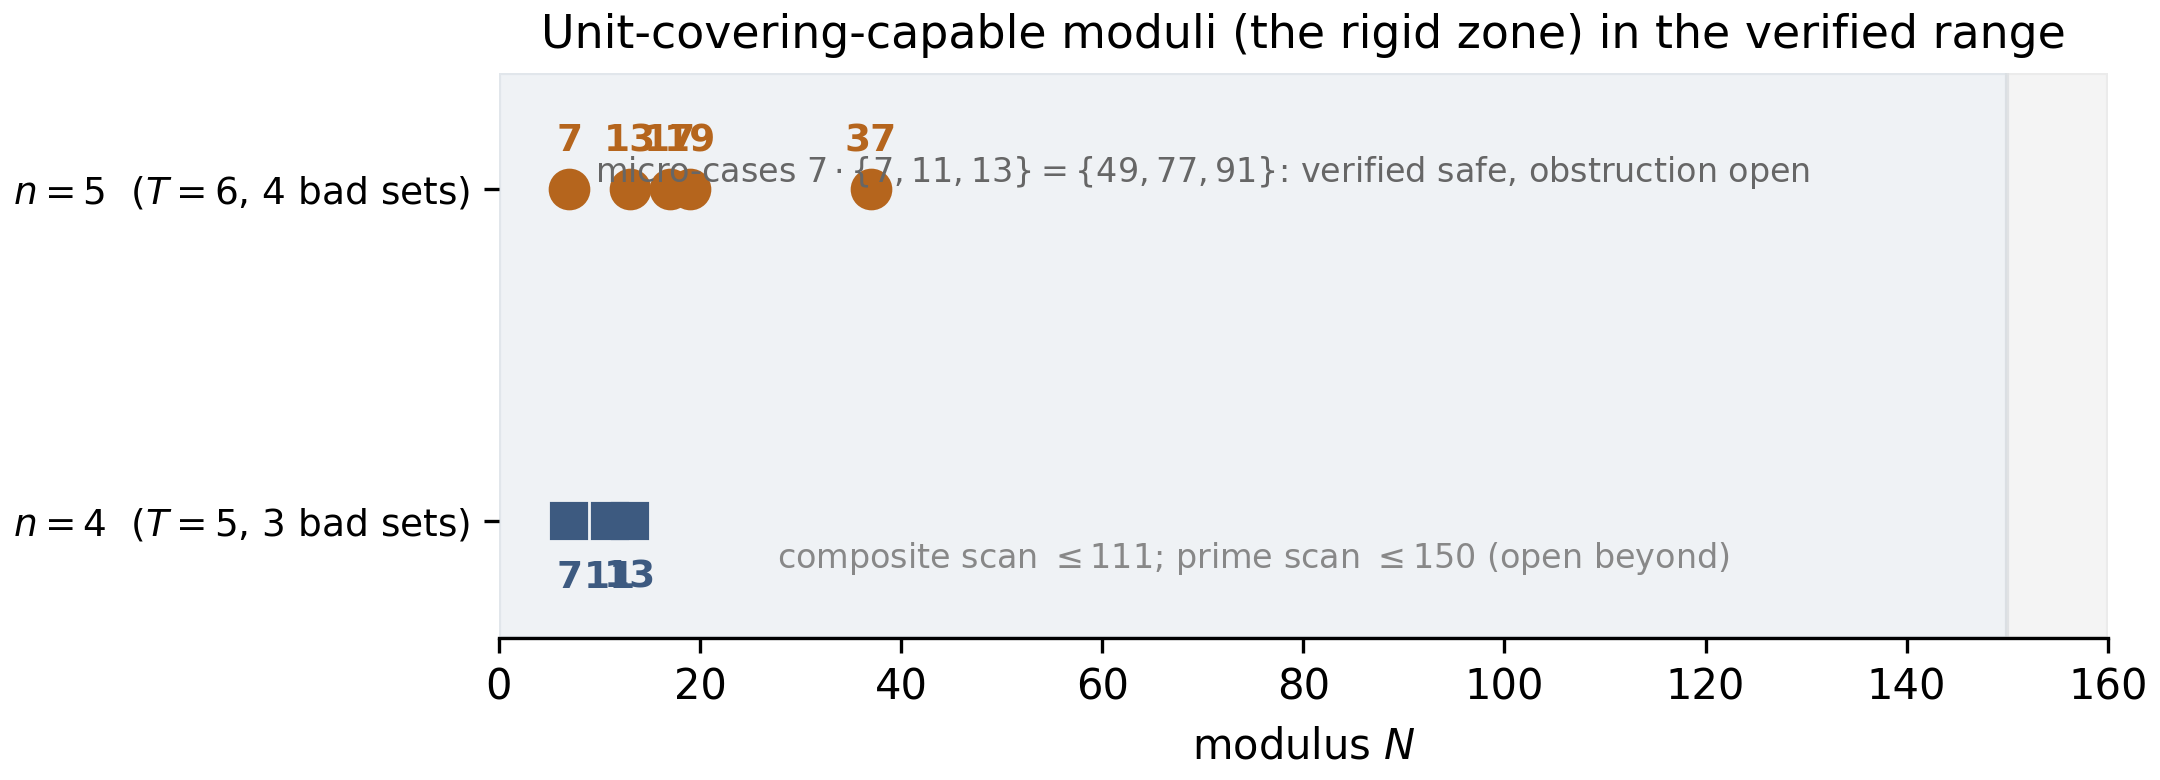
\includegraphics[max width=\textwidth, max height=0.32\textheight]
  {fig_rigidzone.png}
\end{center}

Three features of Table~\ref{tab:rigid} organize this section. First, the
zones are \emph{small and scattered}: no arithmetic progression, no
obvious multiplicative family---$17,19,37$ are not lifts of anything
smaller (they are prime, and prime moduli are their own base by
Lemma~\ref{lem:lift}). Second, the $n=4$ zone does not contain the $n=5$
zone and vice versa: $11$ is capable with three bad sets but not with
four---counting kills it, since four unit bad sets at $N=11$ ($h=1$,
$|B_w|=3$) have union of size at most $4\cdot 3-3=9<11$---while
$17,19,37$ are incapable with three bad sets and capable with four. The
rigid zone is a genuinely rung-dependent object. Third, within the
verified range the $n=5$ zone is \emph{constant} as the range grows:
after $37$, no modulus whatsoever (prime or composite) is capable, through
primes $150$ and composites $111$. We call this the rigid-zone map; it is
an empirical finding, stated with its range, and we emphasize that its
finiteness is not proved (Conjecture~\ref{conj:successor} is the natural
positive statement).

The rest of the section classifies the covering configurations at every
capable prime, at both rungs. The classifications are exact
if-and-only-if theorems; their proofs at $N\le 17$ are group-theoretic
(tilings and matchings), and at $19,37$ rest on an exhaustive finite check
whose verification record is in \S\ref{sec:sound}. Throughout,
$m=(N-1)/2$, $C=\Z_N^\ast/\{\pm1\}\cong\Z_m$, and by
Lemma~\ref{lem:class} a unit tuple covers $\Z_N$ iff the class sets
$X_w\cdot S_h$ cover $C$.

\subsection{The base rung: three bad sets}\label{sec:K4}

\begin{theorem}[$K_7$; $n=4$]\label{thm:K4}
Let $N=7$ ($h=1$, $C\cong\Z_3$). Three unit bad sets cover $\Z_7$ iff
their antipodal classes $\{\pm w_i^{-1}\}$ are the three distinct classes
of $\Z_7^\ast$. There are $4$ scale-normalized covering pairs
$(b,c)$ at $a=1$: $(2,3)$, $(2,4)$, $(3,5)$, $(4,5)$.
\end{theorem}

\begin{proof}
Here $S_h=S_1$ is a single class, so $B_w$ contributes exactly the class
$X_w$, and three bad sets cover iff $\{X_1,X_b,X_c\}=C$. The covering
pairs are read off $\Z_7^\ast$: the classes are
$\{1,6\},\{2,5\},\{3,4\}$; with $a=1$ contributing $\{1,6\}$, the pair
$(b,c)$ must contribute $\{2,5\}$ and $\{3,4\}$, i.e.\
$b\in\{2,5\}$, $c\in\{3,4\}$ with the classes of $b,c$ distinct and
completing $C$---enumerating gives exactly the four listed pairs.
\end{proof}

\begin{theorem}[$K_{11}$: domino adjacency]\label{thm:K11}
Let $N=11$ ($h=2$, $C\cong\Z_5$, generated by $g=\cls(2)$). Each unit
bad set covers the \emph{domino} $\{X_w,X_w g\}$ of $C$. Three dominos
$\{t_i,t_i+1\}$, $t_i\in\Z_5$, cover $C$ iff the complement of the start
set $T=\{t_1,t_2,t_3\}$ (two vertices of $C_5$) contains no adjacent
pair. There are $12$ scale-normalized covering pairs.
\end{theorem}

\begin{proof}
A vertex $p\in C$ is uncovered iff $p\notin T$ and $p-1\notin T$; since
$|T|=3$ and $|C|=5$, covering fails iff the two-element complement
contains an adjacent pair $\{p-1,p\}$. With the scale normalization
$w_1=1$ (so $e(X_1)=0\in T$) the admissible complements are
$\{1,3\},\{1,4\},\{2,4\}$---that is, the start sets
$\{0,2,4\},\{0,2,3\},\{0,1,3\}$---and each is realized by four
multisets $(1,b,c)$ (each of the two remaining starts is realized by two
residues, $b$ and $-b$, with the same class), giving $3\times 4=12$,
matching the direct scan.
\end{proof}

\begin{theorem}[$K_{13}$: coset tiling]\label{thm:K13}
Let $N=13$ ($h=2$, $C\cong\Z_6$, generated by $g=\cls(2)$). Three unit
bad sets cover $\Z_{13}$ iff their start classes $X_w$ form a coset
$\{X,\,Xg^2,\,Xg^4\}$ of the order-$3$ subgroup of $C$. There are $4$
scale-normalized covering pairs: $(3,4)$, $(3,9)$, $(4,10)$, $(9,10)$ at
$a=1$.
\end{theorem}

\begin{proof}
Each bad set covers the domino $\{X_w,X_wg\}$; three dominos on the
$6$-cycle cover iff they are pairwise disjoint (three sets of size two
covering six vertices). Disjointness of $\{t,t+1\}$ and $\{s,s+1\}$ on
$\Z_6$ is equivalent to $s-t\notin\{-1,0,1\}$, i.e.\ $s-t\in\{2,3,4\}$
up to sign. Three starts pairwise at such differences must be
$\{t,t+2,t+4\}$: if two starts differ by $3$, no third start is compatible
(differing from both by $\{2,3,4\}$ mod $6$), and the remaining
possibilities are exactly the cosets of $\{0,2,4\}$. The four listed
pairs are the realizations with $e(X_1)=0$ fixed.
\end{proof}

\subsection{The second rung: four bad sets}\label{sec:K5}

At $n=5$ the same three group-theoretic mechanisms persist at
$7$ and $13$ (now with four dominos: at $N=7$, four classes cover
$C_3$ iff they hit all three classes; at $N=13$, four dominos cover
$C_6$ iff the complement of the start set contains no adjacent pair), and
one new mechanism appears at $17$.

\begin{theorem}[$K_{17}$: perfect matching]\label{thm:K17}
Let $N=17$ ($h=2$, $C\cong\Z_8$; $c=\cls(2)$ has order $4$ since
$2^4\equiv-1 \pmod{17}$). Each unit bad set covers the domino
$\{X_w,X_wc\}$, and dominos live inside the two cosets of the order-$4$
subgroup $\langle c\rangle$, each coset a $4$-cycle under multiplication
by $c$. Four unit bad sets cover $\Z_{17}$ iff each coset contains
exactly two of the four starts and the two are non-adjacent in that
$4$-cycle (equivalently, differ by $c^2$). There are $16$
scale-normalized covering $4$-multisets.
\end{theorem}

\begin{proof}
Within one $4$-cycle $\{x,xc,xc^2,xc^3\}$, two dominos
$\{X,Xc\}$, $\{Y,Yc\}$ cover the cycle iff they are disjoint iff
$Y\notin\{X,Xc,Xc^{-1}\}$, i.e.\ $Y=Xc^2$. If one coset contained three
starts, the other would contain one, and a single domino covers only two
of its cycle's four vertices; if one coset contained all four, the other
would be untouched. Hence exactly two starts per coset, at antipodal
positions of the $4$-cycle. The count of scale-normalized realizations is
$16$, matching the direct scan; the sparsity is the matching constraint.
\end{proof}

\begin{example}[a covering at $17$, by hand]\label{ex:17}
The residues $(1,4,6,7)$ cover $\Z_{17}$:
\[
B_1\cup B_4\cup B_6\cup B_7
=\{0,\pm1,\pm2\}\cup\{0,\pm4,\pm9\}\cup\{0,\pm3,\pm6\}
 \cup\{0,\pm5,\pm10\}=\Z_{17},
\]
the eight classes $\{\pm1,\pm2,\pm4,\pm9,\pm3,\pm6,\pm5,\pm10\}$
exhausting $C_8$. This is realizable as a genuine speed set: the pair
$(1,16)$ of $V=(1,4,6,7,16)$ has effective residues $(1,4,6,7)$ on
$\Z_{17}$ and is a true (non-certifying) pair. Hand-checkable anchors of
this kind anchor every classification to the original problem.
\end{example}

At $N=19$ and $N=37$ the covering radius $h$ reaches $3$ and $6$, the
class segments $S_h$ grow past two elements, and the tiling gloss ends:
the classifications become explicit finite lists. Fix a generator
$g=\cls(2)$ of $C$ (at both moduli $2^{m}\equiv -1$, verified), write
$e(\cls(g)^t)=t$ for the \emph{exponent} of a class, and let
$S=e(S_h)\subseteq\Z_m$. By Lemma~\ref{lem:class}, a unit $4$-tuple
covers $\Z_N$ iff
\[
\bigcup_{i=1}^{4}\bigl(e(X_{w_i})+S\bigr)=\Z_m .
\]
Multiplying all four residues by a unit $u$ shifts every exponent by the
constant $-e(\cls u)$, so covering depends only on the \emph{translate
class} of the exponent multiset in $\Z_m$.

\begin{theorem}[$K_{19}$]\label{thm:K19}
Let $N=19$: $m=9$, $h=3$, $S=\{0,1,4\}$. Four unit bad sets cover
$\Z_{19}$ iff the exponent multiset $\{e(X_{w_i})\}$ is a translate of
\[
A=\{0,1,2,7\}\quad(\text{gaps }1,1,5,2)
\qquad\text{or}\qquad
B=\{0,2,4,6\}\quad(\text{gaps }2,2,2,3),
\]
the latter being the doubled interval $2\cdot\{0,1,2,3\}$. There are
exactly two covering translate classes and $64$ scale-normalized covering
residue $4$-multisets ($8$ residue realizations per class, all with four
distinct exponents).
\end{theorem}

\begin{theorem}[$K_{37}$]\label{thm:K37}
Let $N=37$: $m=18$, $h=6$, $S=\{0,1,2,5,8,9\}$. Four unit bad sets cover
$\Z_{37}$ iff the exponent multiset is a translate of the single class
\[
C_0=\{0,2,12,15\}\quad(\text{gaps }2,10,3,3).
\]
There is one covering translate class and $32$ scale-normalized covering
residue $4$-multisets.
\end{theorem}

\begin{proof}[Proof of Theorems~\ref{thm:K19} and \ref{thm:K37}]
The reduction to translate classes is proved above. The class lists are
then decided by exhaustive enumeration of all contains-$0$ $4$-multisets
of $\Z_m$ ($165$ candidates at $m=9$, $1{,}140$ at $m=18$---hand-checkable
scale), checking $\bigcup(e_i+S)=\Z_m$ exactly. Correctness of the
packaging was verified bidirectionally against the residue level: over
\emph{all} unit $4$-multisets ($5{,}985$ at $N=19$, $82{,}251$ at
$N=37$), the predicate ``exponent multiset is a translate of a listed
class'' agrees with direct bitmask covering, with zero mismatches in
either direction; the residue covering counts $64$ and $32$ were
reproduced by three independent implementations (bitmask, frozenset,
exponent-space). The full verification record is in \S\ref{sec:sound}.
\end{proof}

\begin{remark}[what the classifications say structurally]\label{rem:pattern}
Three structural facts deserve the reader's attention, because they are
the paper's central finding. First, \emph{every covering configuration at
every rigid prime has four distinct antipodal classes}: no covering
multiset repeats an exponent. This is consistent with
Lemma~\ref{lem:D3}: $19\equiv 1\pmod 6$ is exactly the case its $p_m=3$
bound cannot reach, and the classification shows covering there needs the
full $p_m=4$. Second, \emph{negation is not a symmetry} of the covering
problem: $B_{-w}=B_w$, so the negated tuple $(-w_i)$ is a genuinely
different tuple whose classes differ; the negation class of $B=\{0,2,4,6\}$
happens to be covering (it is negation-stable) while those of $A$ and
$C_0$ are not---negation acts as a diagnostic, never as an invariance,
and an earlier attempt to quotient by it was discarded as unsound. Third,
the character of the classification changes at $h\ge 3$: $K_{13}$ and
$K_{17}$ are group-theoretic statements (tilings, matchings) with slick
proofs, while $K_{19}$ and $K_{37}$ are finite lists. The classification
is complete but the tiling gloss does not persist---we read this as a
genuine change in the texture of the landscape, not as a gap in the
method.
\end{remark}

\subsection{Composite moduli}\label{sec:composites}

Composites split cleanly by parity (Proposition~\ref{prop:reach}): even
composites are never unit-capable, and odd composites are governed by the
reachability mechanism---a covering by unit bad sets must cover every
non-unit class, but unit bad sets reach non-unit classes only through
$j\le h$ with $\gcd(j,N)>1$. Table~\ref{tab:composites} records the
outcome for every odd composite in the open part of the range
($49$--$111$): a \emph{proved} safety whenever some non-unit class is
unreachable, and a handful of \emph{micro-cases} where all non-unit
classes are reachable, the slot counts do not obstruct, and no \emph{unit}
covering exists anyway (Table~\ref{tab:composites}; the qualification
``unit'' is load-bearing --- see Remark~\ref{rem:postcomposite}).

\begin{table}[htbp]
\centering
\small
\caption{Odd composites $49$--$111$ at $n=5$ ($T=6$): non-unit antipodal
classes, how many are reachable by unit bad sets (via
$j\le h$, $\gcd(j,N)>1$), and capability. All entries cross-checked by an
independent set-based scanner; zero capable moduli.}
\label{tab:composites}
\begin{tabular*}{\textwidth}{@{\extracolsep{\fill}} r r r r l}
\toprule
$N$ & $h$ & non-unit classes & reachable & status \\
\midrule
$49=7^2$      & 8  & 3  & \textbf{3} & micro-case (verified safe) \\
$51=3\cdot17$ & 8  & 9  & 8  & proved safe \\
$55=5\cdot11$ & 9  & 7  & 5  & proved safe \\
$57=3\cdot19$ & 9  & 10 & 9  & proved safe \\
$63$          & 10 & 13 & 12 & proved safe \\
$65=5\cdot13$ & 10 & 8  & 6  & proved safe \\
$69$          & 11 & 12 & 11 & proved safe \\
$75$          & 12 & 17 & 14 & proved safe \\
$77=7\cdot11$ & 12 & 8  & \textbf{8} & micro-case (verified safe) \\
$81=3^4$      & 13 & 13 & 12 & proved safe \\
$85=5\cdot17$ & 14 & 10 & 8  & proved safe \\
$87=3\cdot29$ & 14 & 15 & 14 & proved safe \\
$91=7\cdot13$ & 15 & 9  & \textbf{9} & micro-case (verified safe) \\
$93=3\cdot31$ & 15 & 16 & 15 & proved safe \\
$95=5\cdot19$ & 15 & 11 & 9  & proved safe \\
$99=9\cdot11$ & 16 & 19 & 18 & proved safe \\
$105=3\cdot5\cdot7$ & 17 & 28 & 25 & proved safe \\
$111=3\cdot37$ & 18 & 19 & 18 & proved safe \\
\bottomrule
\end{tabular*}
\end{table}

The micro-cases form a pattern too clean to be coincidence:
\[
49=7\cdot 7,\qquad 77=7\cdot 11,\qquad 91=7\cdot 13,
\]
that is, the products of $7$ with the $n=4$ rigid-zone primes
$\{7,11,13\}$. These are precisely the odd composites in range where
\emph{every} non-unit class is reachable, so the reachability mechanism is
silent, yet no unit covering exists; the obstruction is multiplicative.
The pattern predicts that the next
micro-cases, if any, should be sought at $7\cdot17=119$ and $7\cdot19=133$
(and $7\cdot37=259$), all outside the scanned composite range. We flag
this as an open problem (\S\ref{sec:open}) rather than a conjecture: three
data points do not make one.

\begin{remark}[post-submission development at the composite moduli]
\label{rem:postcomposite}
Work completed after this manuscript was assembled (companion note) changes
the micro-case picture in three ways, and the open problem is restated
accordingly in \S\ref{sec:open}. First, the \emph{fibration}: a bad set
whose speed has $d=\gcd(w,N)>1$ is the full preimage of a unit bad set at
$N/d$ with the \emph{same} threshold. Consequently kernel-speed coverings
\emph{do} exist at the micro-cases --- for example
$B_7\cup B_{14}\cup B_{21}=\Z_{49}$ is the transferred $K_7$ classification
--- so ``no covering at composites'' is false as a blanket statement; what
the micro-cases exclude is unit coverings, and more generally any covering
in which units are load-bearing. Second, the unit-side statement that
survives is \emph{no unit assistance}: at $N=p^2$ and $N=pq$ with
$p\ge5$, a covering family of at most four distinct bad sets with at most
two unit members has its kernel subfamily covering; three unit bad sets
never cover at all for $N\ge31$, $N\not\equiv0\pmod6$; and a pure-unit
family covers only above rigid-zone primes --- which makes the unit safety
of $77=7\cdot11$ a theorem rather than a verification (its reduction
demands a covering of $\Z_{11}$, and $11$ is not in the $n=5$ zone). Third,
the residual is explicit: the cells with three unit sets and at most one
kernel set, occupied at $N=9$ (a genuine unit-assisted covering, and the
reason the prime hypothesis cannot be dropped), verified empty at $p=5$
and throughout the tested composite range.

\medskip
Fourth (the $p^2$ closure, completing the companion note's programme):
the last open cell at square moduli --- one kernel set with three unit
sets --- is now \emph{empty at every prime $p\ge5$}.  For unit triples
whose residues are pairwise $\pm$-distinct mod $p$, the trichotomy
programme applies: Lemma~B ($p\equiv5\pmod6$) is proved for $p\ge17$
(the kills run on the contained census, Lemma T, clean from $p=17$, and
Corollaries T1--T3; a pre-T3 draft of the overlap kill had required
$p\ge23$), with $p=11$ closed by exhaustive finite case analysis (36
viable configurations, each carrying a positive residual-fit margin of at
least $2$, cross-validated by an independent brute force that reproduces
the known failure counts $50$ at $p=7$ and $2$ at $p=13$ exactly, the
$p=17$ finite analysis of the earlier draft now a redundant
verification); Lemma~A ($p\equiv1\pmod6$) is proved for $p\ge31$
unconditionally --- its one remaining input, the foot-count trichotomy
in its consumed form (the one-foot statement at the two size pairs
$(2k{+}2,2k{+}1)$ and $(2k{+}1,2k{+}1)$, viable differences confined to
$\{2,(p-1)/2\}$), is discharged by Lemma~\ref{lem:E} of
\S\ref{sec:lemmaE} (the three-distance foot count, proved for every
$p\ge31$ and cross-checked against the foot census of the previous
revision to $p\le419$) --- with $p=19$ closed the same way (614
viable configurations, margin $3$), and it is \emph{false} at $p=7,13$,
where $\pm$-distinct coverings exist and the cells are closed by direct
verification. For $\pm$-colliding units ---
two speeds equal up to sign mod $p$, a configuration the cell definition
does not exclude and the trichotomy lemmas do not reach --- a new argument
closes the case: the two colliding bad sets are shears of one another, so
their per-fiber $t$-space placements drift \emph{exactly linearly} in the
fiber index, while the fiber covering configurations are pinned (the
placements' difference set has at most $6$ elements, with covering counts
$28$ and $68$ per collision topology, \emph{independent of $p$}); a
pigeonhole over the $p-|B_k|$ kernel-uncovered fibers then kills every
family.  The mechanism is proved in general; its computational input is
stated as a named lemma with its verification range (every prime
$11\le p\le 113$), and the ground truth is an exhaustive enumeration of
$3.3$\,million colliding families at $p\le43$ with zero coverings, the
nearest families failing all but two fibers.

The closure's exact dependency structure is now recorded in
\S\ref{sec:groupring}, and it is sharper than ``modulo two computational
inputs'': of the two named inputs, one is now \emph{proved} --- the
foot-count inequality for the one-foot trichotomy (in the consumed form,
clean from $p\ge31$) is Lemma~\ref{lem:E} of \S\ref{sec:lemmaE}, an
elementary three-distance argument with no group-ring content --- so the
closure rests on a single unbounded hypothesis, the four-family covering
classification for the pinning lemma (verified to $p\le113$, and
subsuming the shear-rigidity input because the pinned per-fiber
configurations are exactly the classified families). The $pq$
side of \S\ref{sec:pq} now carries the same structure at semiprime moduli:
the $(1,1,2)$ and three-unit cells at $N=pq$ are verified empty to
$N\le143$ and reduce, by the row translation, to exactly the same
remaining input.
\end{remark}

\subsection{Discharging Input E: the three-distance foot count}\label{sec:lemmaE}

Input E in its consumed form (\S\ref{sec:gt-support}) is the one-foot
trichotomy at the two size pairs consumed by the kills M4 and M5 of
Lemma~A: at $p=6k+1$, an arithmetic progression $A(a,d,s)$ of critical
size $s\in\{2k{+}1,2k{+}2\}$ with at most one point outside
$I_1=[s_1,p-1]$ (where $(s_1,s)=(2k{+}2,2k{+}1)$ for M4 and
$(2k{+}1,2k{+}1)$ for M5) must have $\|d\|\in\{2,(p-1)/2\}$. This
subsection proves that statement outright for every prime $p\ge31$
(Lemma~\ref{lem:E} below) --- the discharge route identified in
\S\ref{sec:gt-support}, carried out by an elementary, self-contained
analysis of the rotation $j\mapsto jd\bmod p$: the three-distance
theorem of that rotation, in exactly the regime the consumers need. No
group-ring input is used. Throughout, $p=6k+1$ is prime, $3k=(p-1)/2$,
and $d$ is a $\pm$-representative in $[2,3k]$.

\paragraph{Notation.} For $s\ge2$ put
$X=X^{(s)}_d=\{jd\bmod p:0\le j<s\}$ (so $A(a,d,s)=a+X$), let
$x_1<\dots<x_s$ be its sorted elements and $g_i=x_{i+1}-x_i$ for $i<s$,
$g_s=p-x_s+x_1$ its cyclic gaps; the pair sums $g_i+g_{i+1}$ (indices
mod $s$) are the spans $\mathrm{next}(x)-\mathrm{prev}(x)$ over $x\in
X$, and $G_2(X)=\max_i(g_i+g_{i+1})$. Recall
$\mathrm{feet}(A)=s-|A\cap I_1|$, the number of points of $A$ in
$[0,s_1)$. For $R\subseteq\Z_n$ with $0\in R$, sorted
$0=\rho_1<\dots<\rho_t$, let $\Gamma_2(R;n)$ be the largest sum of
cyclically adjacent gaps of $R$ on $\Z_n$ (the last gap being
$n-\rho_t$; $t=1$: $\Gamma_2=2n$), and write
$\gamma^{\mathrm f}(R)=\rho_2$ (first gap) and
$\gamma^{\mathrm w}(R;n)=n-\rho_t$ (wrap gap).

\begin{lemma}[feet and pair sums]\label{lem:E0}
For $X\subseteq\Z_p$ with $|X|\ge2$ and $2\le L\le p$: every cyclic
interval of $L$ consecutive residues meets $X$ in at least two points
iff $G_2(X)\le L$. In particular,
$\min_a\mathrm{feet}(A(a,d,s))\ge2$ iff $G_2(X^{(s)}_d)\le s_1$.
\end{lemma}

\begin{proof}
An $L$-interval $[u,u+L)$ contains at most one point of $X$ iff some
$x\in X$ has $\mathrm{prev}(x)<u$ and $u+L\le\mathrm{next}(x)$: for the
unique point of a one-point instance this is immediate, and for an empty
instance it holds with $x$ the first point at or after $u+L$. Either
way $\mathrm{span}(x)\ge L+1$; conversely a point of span $\ge L+1$
produces the one-point interval $[\mathrm{prev}(x)+1,\,
\mathrm{prev}(x)+L+1)$. For the second claim,
$\#(a+X)\cap[0,s_1)=\#X\cap([0,s_1)-a)$, and $([0,s_1)-a)$ runs through
all cyclic $s_1$-intervals as $a$ does.
\end{proof}

\begin{lemma}[column decomposition]\label{lem:E1}
Let $s\in\{2k{+}1,2k{+}2\}$, $2\le d\le3k$, and
$W=\floor{d(s-1)/p}\ge1$; write $r=p\bmod d$, $\sigma=d-r$,
$m_0=\floor{p/d}$, and $c_w=(-wp)\bmod d\in[0,d)$ for $0\le w\le W$.
Then: \textup{(i)} $c_0,\dots,c_W$ are distinct; \textup{(ii)} the $j$
with $\floor{dj/p}=w$ form the interval
$[\lceil wp/d\rceil,\,\min(\lceil(w{+}1)p/d\rceil-1,\,s-1)]$, and the
corresponding points $jd\bmod p=dj-wp$ are exactly
$c_w,c_w+d,\dots,c_w+(h_w-1)d$, where
$h_w=\lceil(w{+}1)p/d\rceil-\lceil wp/d\rceil$ for $w<W$ and
$h_W=s-\lceil Wp/d\rceil$; \textup{(iii)} for $w<W$ the run is the
\emph{full} column $\{x\in[0,p):x\equiv c_w\pmod d\}$ --- of height
$F(c)=m_0+1$ for $c<r$ and $m_0$ otherwise, with top $p-d+c_{w+1}$ ---
while run $W$ is the prefix of the column of $c_W$ of height
$h_W\le F(c_W)$, with top $H=d(s-1)-Wp$.
\end{lemma}

\begin{proof}
(i) $p$ is prime and $d<p$, so $\gcd(p,d)=1$; and
$W\le d(s-1)/p\le d(2k+2)/(6k+1)<d$, so $w\mapsto wp\bmod d$ is
injective on $[0,W]$. (ii) $\floor{dj/p}=w$ iff $wp\le dj<(w+1)p$, i.e.\
$j\in[\lceil wp/d\rceil,\lceil(w+1)p/d\rceil-1]$, truncated at $s-1$;
the sequence $\floor{dj/p}$ increases in steps of $0$ or $1$ (as $d<p$),
so every $w\le W$ occurs. The first point of run $w$ is
$d\lceil wp/d\rceil-wp\in[0,d)$ with residue $\equiv-wp\equiv c_w$, so
it equals $c_w$; the run then steps by $d$ within its column. (iii) For
$w<W$ the last point is
$d(\lceil(w{+}1)p/d\rceil-1)-wp=p-d+\beta_w$, where
$\beta_w=d\lceil(w{+}1)p/d\rceil-(w{+}1)p\in[0,d)$ is the canonical
representative of $c_{w+1}$. This top lies in $[p-d,p)$ and satisfies
$p-d+\beta_w\equiv r+c_{w+1}\equiv c_w\pmod d$ (since
$c_{w+1}\equiv c_w+\sigma$ and $r+\sigma=d$); being congruent to $c_w$
and in $[p-d,p)$ it is the top of the full column of $c_w$, whose
$F(c)=\lceil(p-c)/d\rceil$ elements are $c,c+d,\dots$ --- so run $w$ is
that full column and $h_w=F(c_w)$. Run $W$ spans
$j\in[\lceil Wp/d\rceil,s-1]$, hence is the bottom prefix of height
$h_W=s-\lceil Wp/d\rceil\le F(c_W)$, with top $d(s-1)-Wp$.
\end{proof}

\begin{lemma}[bands and the pair-sum identity]\label{lem:E2}
In the setting of Lemma~\ref{lem:E1} with $W\ge1$, put
$C=\{c_0,\dots,c_W\}$, $C^-=C\setminus\{c_W\}$, $h=h_W$, and
$T=(C^-\cap[0,r))\cup E$ with $E=\{c_W\}$ if $h>m_0$ and $E=\emptyset$
otherwise. Then:
\textup{(i)} for $0\le i\le m_0$, the residues of $X$ in the band
$[id,(i{+}1)d)$ are exactly $R_i=C$ if $i<h$, $R_i=C^-$ if
$h\le i\le m_0-1$, and $R_{m_0}=T$; in particular
$R_0\supseteq\dots\supseteq R_{m_0}$, all containing $0$;
\textup{(ii)} the gap sequence $(g_1,\dots,g_s)$ is the concatenation,
over $i=0,\dots,m_0-1$, of the cyclic gap block of $R_i$ on $\Z_d$
(consecutive differences of $R_i$, ending with the wrap gap
$d-\max R_i$), followed by the top block of $T$ (consecutive
differences, ending with $r-\max T$);
\textup{(iii)} the pair sums of $X$ are the cyclic two-step gaps of
these blocks --- a singleton band contributing the double wrap $2d$,
attained iff the band below is also a singleton; singleton bands occur
only for $W=1$ --- together with the boundary pairs
$\gamma^{\mathrm w}(R_{i-1};d)+\gamma^{\mathrm f}(R_i)$ (reading
$\gamma^{\mathrm f}=d$ for a singleton band), of which those with
$i\le m_0-1$ are at most $\gamma^{\mathrm w}(R_i;d)+\gamma^{\mathrm
f}(R_i)\le\Gamma_2(R_i;d)$ by (i), together with the two outer pairs
\[
\mathrm{span}_0=(r-\max T)+\gamma^{\mathrm f}(C),\qquad
\mathrm{span}^\ast=(d-\max R_{m_0-1})+\begin{cases}
\gamma^{\mathrm f}(T)&|T|\ge2,\\ r&|T|=1.\end{cases}
\]
Consequently, for $W\ge2$,
\[
G_2(X)=\max\bigl(\Gamma_2(C;d),\ \Gamma_2(C^-;d)\ \text{[if $h\le
m_0-1$]},\ \Gamma_2(T;r)\ \text{[if $|T|\ge2$]},\
\mathrm{span}_0,\ \mathrm{span}^\ast\bigr),
\]
while for $W=1$, $G_2(X)\le2d$.
\end{lemma}

\begin{proof}
(i) By Lemma~\ref{lem:E1}, $X$ is the union of the runs, run $w$
occupying bands $0,\dots,h_w-1$ at residue $c_w$. For $i\le m_0-1$ every
full run is present ($h_w=F(c_w)\ge m_0>i$), and run $W$ is present iff
$h>i$; hence $R_i=C$ for $i<h$ and $C^-$ otherwise. Band $m_0$ sees
exactly the full runs with $F(c_w)>m_0$, i.e.\ $c_w<r$, plus run $W$ iff
$h>m_0$: that is $T$. The nesting is immediate, and $0=c_0\in C^-$ (as
$W\ge1$) with $0<r$ puts $0$ in every band. (ii) Band $i$'s points, in
increasing order, are $c+id$ with $c\in R_i$ in residue order, so the
within-band gaps are the residue differences; the gap from band $i$'s
last point to band $i{+}1$'s first (residue $0$, since $0\in
R_{i+1}$) is $d-\max R_i$; and the final wrap, from $\max T+m_0d$ to
$0$, is $r-\max T$ (as $p=m_0d+r$). (iii) The pair sum around a point
of band $i$ is either within-block (a two-step gap of $R_i$; around the
band's last point it is the last two gaps of the block, equally a
two-step gap) or crosses the boundary below, where it is the last gap
of block $i-1$ plus the first gap of block $i$; for $i\le m_0-1$ the
nesting (i) gives $\gamma^{\mathrm w}(R_{i-1};d)\le\gamma^{\mathrm
w}(R_i;d)$, and the wrap and first gaps are cyclically adjacent, so the
boundary pair is at most $\Gamma_2(R_i;d)$. A singleton band $R_i=\{0\}$
arises only when $C^-=\{0\}$, i.e.\ $W=1$; its lone point has pair sum
$\gamma^{\mathrm w}(R_{i-1};d)+d$, which equals $2d$ exactly when
$R_{i-1}=\{0\}$ as well. The top band contributes the two-step gaps of
$T$ on $[0,r)$ (only for $|T|\ge2$; around $T$'s last point the pair is
the last within-gap plus $r-\max T$, again a two-step gap on $\Z_r$),
the boundary pair $\mathrm{span}^\ast$ around $m_0d$, and --- around
$0$ --- the outer pair $\mathrm{span}_0$. For $W\ge2$ no band is a
singleton ($|C^-|=W\ge2$), so every pair sum is at most the maximum of
the five displayed quantities; conversely each of the five is realized
as a pair sum of $X$ ($\Gamma_2(C)$ in band $0$; $\Gamma_2(C^-)$ in a
$C^-$-band, which exists exactly when $h\le m_0-1$; $\Gamma_2(T;r)$ in
the top band; $\mathrm{span}_0$ around $0$; $\mathrm{span}^\ast$ around
$m_0d$). For $W=1$: $\Gamma_2(C;d)=d$, the singleton-band terms are at
most $2d$, $\mathrm{span}_0\le d$, and $\mathrm{span}^\ast<2d$: if $|T|=1$
then $R_{m_0-1}\in\{C,C^-\}$ gives $(d-\sigma)+r=2r$ resp.\ $d+r$,
both $<2d$; if $|T|=2$ then $h=m_0+1$, $R_{m_0-1}=C$, and
$(d-\sigma)+\gamma^{\mathrm f}(T)<(d-\sigma)+r=d$. Hence $G_2\le2d$.
\end{proof}

\begin{lemma}[wrap count]\label{lem:E3}
For $k\ge2$ and $s=2k{+}1$: $W\ge d-2k+1$ for $3\le d\le3k-2$, $W=d-2k$
at $d=3k-1$, and $W=d-2k-1$ at $d=3k$. For $s=2k{+}2$: $W\ge d-2k+1$
for $3\le d\le3k-2$, and $W=d-2k$ at $d\in\{3k-1,3k\}$.
\end{lemma}

\begin{proof}
Since $d-2k+1$ is an integer, $W=\floor{d(s-1)/p}\ge d-2k+1$ iff
$d(s-1)\ge(d-2k+1)p$, a quadratic inequality in $d$. For $s=2k+1$ it
reads $d(4k+1)\le12k^2-4k-1$, i.e.\
$d\le3k-1-\frac{3k}{4k+1}<3k-1$, so it holds for $d\le3k-2$ --- for
$d\le2k$ trivially, since then $d-2k+1\le1\le W$ (with $W=0\ge4-2k$ at
$d=3$, and $W\ge1$ for $d\ge4$). The endpoint values are direct:
$W=\floor{2k(3k-1)/(6k+1)}=k-1=d-2k$ and $W=\floor{6k^2/(6k+1)}=k-1$.
For $s=2k+2$ the inequality reads $4kd\le12k^2-4k-1$, i.e.\
$d\le3k-1-\frac1{4k}$, again $d\le3k-2$ (for $d\le2k$ trivially:
$d-2k+1\le1\le W$, $W\ge1$ for $d\ge3$), with endpoints
$W=\floor{(2k+1)(3k-1)/(6k+1)}=k-1$ and
$W=\floor{3k(2k+1)/(6k+1)}=k$.
\end{proof}

\begin{lemma}[auxiliary bounds]\label{lem:E4}
In the setting of Lemmas~\ref{lem:E1}--\ref{lem:E2}:
\textup{(a)} for $R\subseteq\Z_n$ with $0\in R$ and $2\le|R|\le n$,
$\Gamma_2(R;n)\le n-|R|+2$;
\textup{(b)} if $d\le3k-1$ then $r\le2k-1$;
\textup{(c)} $\max C\le\max T+\sigma$;
\textup{(d)} $\mathrm{span}_0\le\Gamma_2(C;d)$;
\textup{(e)} if $W\ge2$ then $\mathrm{span}^\ast\le d-W+2$.
\end{lemma}

\begin{proof}
(a) Let $t=|R|$ and let the cyclic gaps be $\gamma_1,\dots,\gamma_t$
(summing to $n$, each $\ge1$). Every two-step gap is
$\gamma_i+\gamma_{i\pm1}\le\gamma_{\max}+\gamma'$, where $\gamma'$ is
the largest of the other $t-1$ gaps and hence at most
$(n-\gamma_{\max})/(t-1)$; the map $\gamma\mapsto\gamma+(n-\gamma)/(t-1)$
is increasing (constant when $t=2$), and
$\gamma_{\max}\le n-t+1$ by the pigeonhole principle, so
$\Gamma_2\le(n-t+1)+1=n-t+2$.
(b) If $d\le2k$ then $r\le d-1$; if $2k+1\le d\le3k-1$ then
$2d\le6k-2<p$ and $3d\ge6k+3>p$, so $m_0=2$ and
$r=p-2d\le6k+1-4k-2=2k-1$.
(c) The orbit moves by $c_{w+1}=c_w+\sigma$ when $c_w<r$ (no wrap:
$c_w+\sigma<r+\sigma=d$) and by $c_{w+1}=c_w-r$ when $c_w\ge r$; hence
any orbit point $x\ge\sigma$ is $c_w+\sigma$ with $c_w=x-\sigma\in[0,r)$.
If moreover $x\ne c_W$ then $c_w\in C^-\cap[0,r)\subseteq T$, so
$x\le\max T+\sigma$; for $x=c_W\ge\sigma$ the same argument uses
$c_{W-1}=c_W-\sigma\in C^-\cap[0,r)\subseteq T$ ($W\ge1$, so $c_{W-1}$
exists). An orbit point $x$ with $r\le x<\sigma$ (possible only when
$\sigma>r$) satisfies $x<\sigma\le\max T+\sigma$; a point of
$C^-\cap[0,r)$ is at most $\max T$; and $c_W<\sigma$, $x=0$ are
immediate. So every $x\in C$ has $x\le\max T+\sigma$.
(d) By (c), $r-\max T=(d-\sigma)-\max T\le d-\max
C=\gamma^{\mathrm w}(C;d)$; the wrap and first gaps are cyclically
adjacent, so $\mathrm{span}_0\le\gamma^{\mathrm w}(C;d)+\gamma^{\mathrm
f}(C)\le\Gamma_2(C;d)$.
(e) Reflect the orbit: $C\setminus\{0\}=\{d-m:m\in M\}$ with
$M=\{wr\bmod d:1\le w\le W\}$, and $C^-\setminus\{0\}=\{d-m:m\in M^-\}$
with $M^-=\{wr\bmod d:1\le w\le W-1\}$; thus $d-\max C=\min M=:\mu\le
\min M^-=:\mu^-$, so $d-\max R_{m_0-1}$ is $\mu$ or $\mu^-$, and the
elements of $T\setminus\{0\}$ are reflections $d-m$ of multiples
$m\in(d-r,\,d)$. If $|T|=1$: no multiple of $M^-$ lies in $(d-r,d)$
(its reflection would lie in $C^-\cap(0,r)\subseteq T\setminus\{0\}$),
so the $W-1$ distinct integers of $M^-$ lie in $[1,d-r]$ and
$\mu^-\le(d-r)-(W-2)=d-W+2-\sigma$, whence
$\mathrm{span}^\ast\le\mu^-+r\le d-W+2$. If $|T|\ge2$, let
$t=\gamma^{\mathrm f}(T)=\min(T\setminus\{0\})$. When $t\in C^-$: no
multiple of $M^-$ lies above $m_t=d-t$ (its reflection would lie in
$C^-\cap(0,t)$, below $t$), so $M^-\subseteq[\mu^-,m_t]$ gives
$m_t\ge\mu^-+W-2$ and
$\mathrm{span}^\ast\le\mu^-+(d-m_t)\le d-W+2$. When $t=c_W$ (which
forces $h>m_0$ and $c_W<r$, i.e.\ $m_W=d-c_W\in(d-r,d)$, and
$R_{m_0-1}=C$): no multiple at all lies above $m_W$ (a smaller-index
one would reflect into $C^-\cap(0,c_W)$ below $t$, and index $W$ is
$m_W$ itself), so $M\subseteq[\mu,m_W]$ gives $m_W\ge\mu+W-1$ and
$\mathrm{span}^\ast=\mu+(d-m_W)\le d-W+1$.
\end{proof}

\begin{lemma}[three-distance foot count; Input E discharged]\label{lem:E}
Let $p=6k+1$ be prime with $k\ge5$, let $d\in[3,3k-1]$, and let
$s\in\{2k{+}1,2k{+}2\}$. Then $G_2(X^{(s)}_d)\le2k+1$. Consequently, at
both consumer pairs $(s_1,s)=(2k{+}2,2k{+}1)$ and $(2k{+}1,2k{+}1)$,
$\min_a\mathrm{feet}(A(a,d,s))\ge2$ for every $d\in[3,3k-1]$: the
one-foot viable set is contained in $\{2,(p-1)/2\}$, which is Input E
in its consumed form, and Lemma~A is proved for $p\ge31$.
\end{lemma}

\begin{proof}
\emph{Case $W=0$.} Only $d=3$, $s=2k{+}1$: $X=\{0,3,\dots,6k\}$ has
gaps $3,\dots,3,1$, pair sums $6$ and $4$; $G_2=6\le2k+1$.
\emph{Case $W=1$.} Then $p\le d(s-1)<2p$, which at $s=2k{+}1$ gives
$d\in\{4,5,6\}$ and at $s=2k{+}2$ gives $d\in\{3,4,5\}$; by
Lemma~\ref{lem:E2}(iii), $G_2\le2d$. If $d\le5$ then
$G_2\le10\le2k+1$ (as $k\ge5$). If $d=6$ (so $s=2k{+}1$): here $r=1$,
$m_0=k$, and $h=s-F(0)=k$, so no band is a singleton, $T=\{0\}$,
$\mathrm{span}^\ast=2r=2$, and $G_2\le\max(d,\mathrm{span}_0\le d,
\mathrm{span}^\ast)=6\le2k+1$.
\emph{Case $W\ge2$, $d\le3k-2$.} Lemma~\ref{lem:E3} gives
$W\ge d-2k+1$, and no band is a singleton (that would force
$C^-=\{0\}$, i.e.\ $W=1$). Lemma~\ref{lem:E2}(iii) and
Lemma~\ref{lem:E4} bound each candidate:
$\Gamma_2(C;d)\le d-W+1\le2k$ (Lemma~\ref{lem:E4}(a) with $|C|=W+1$);
$\Gamma_2(C^-;d)\le d-W+2\le2k+1$ (same, $|C^-|=W\ge2$; only if it
occurs); $\Gamma_2(T;r)\le r-|T|+2\le r\le2k-1$
(Lemma~\ref{lem:E4}(a),(b); only if $|T|\ge2$);
$\mathrm{span}_0\le\Gamma_2(C;d)\le2k$ (Lemma~\ref{lem:E4}(d));
$\mathrm{span}^\ast\le d-W+2\le2k+1$ (Lemma~\ref{lem:E4}(e)). Hence
$G_2\le2k+1$.
\emph{Case $d=3k-1$.} Here $r=3$, $\sigma=3k-4$, $W=k-1$
(Lemma~\ref{lem:E3}), and, since $p\equiv3\pmod d$,
$c_w=(-3w)\bmod d$; as $3w\le3k-3<d$ for $w\le k-1$,
$C=\{0\}\cup\{d-3w:1\le w\le k-1\}=\{0,2,5,\dots,3k-4\}$, an
arithmetic progression with difference $3$ together with $0$, with
cyclic gaps $2,3,\dots,3$ and $\Gamma_2(C;d)=6$. Full columns have
$F(0)=3$ and $F(c)=2$ for $c\ge3$, so
$\sum_{c\in C^-}F(c)=3+2(k-2)=2k-1$ and $h=s-(2k-1)\in\{2,3\}$: in
either case $h\ge m_0=2$, so $C^-$ never occurs as a band set;
$T=\{0\}$ (at $s=2k{+}1$) resp.\ $T=\{0,2\}$ (at $s=2k{+}2$);
$\Gamma_2(T;3)\le3$; $\mathrm{span}_0\le3+2=5$;
$\mathrm{span}^\ast=(d-\max C)+r=3+3=6$. So $G_2=6\le2k+1$.
Finally, the primes $6k+1$ with $k\le4$ are $7,13,19$ ($25$ is not
prime); at $p=7$ the range $[3,3k-1]$ is empty, and $13,19$ are
Lemma~A's finite-cased primes, so $k\ge5$ is exactly $p\ge31$. The
consequence on viable sets follows from Lemma~\ref{lem:E0} together
with the endpoint values recorded in Remark~\ref{rem:Esharp}.
\end{proof}

\begin{remark}[endpoints and sharpness]\label{rem:Esharp}
The two excluded differences carry exact values. First,
$G_2(X^{(2k+1)}_2)=2k{+}3$: the progression $\{0,2,\dots,4k\}$ has gaps
$2,\dots,2,2k{+}1$, and the two outer pair sums are $2k+3$. Second,
$G_2(X^{(s)}_{3k})=2k{+}2$ for both $s$: at $s=2k{+}1$ through
$\Gamma_2(C;d)$ with $C=\{0\}\cup\{2k{+}1,\dots,3k-1\}$; at
$s=2k{+}2$ through $\Gamma_2(C^-;d)$ with
$C^-=\{0\}\cup\{2k{+}1,\dots,3k-1\}$, which occurs since then $h=1$
--- in both cases the dead residue run $[1,2k]$ plus one cluster gap.
Meanwhile $G_2(X^{(2k+1)}_{3k-1})=6$ (the case $d=3k-1$ above). These
are exactly the one-foot exceptions $\{2,(p{-}1)/2\}$ of the consumed
form. The clean threshold is sharp: at $d=5$ every $p\ge31$ has
$G_2=2d=10$ (the two-column case with two consecutive singleton bands:
$m_0-h=2\floor{(6k+1)/5}-2k\ge2$ for $k\ge4$), and $10\le2k+1$ first
holds at $k=5$, i.e.\ $p=31$; at $p=19$ the dirty differences are
$d\in\{4,5\}$, each with $G_2=8$ ($2d=8$ resp.\
$\mathrm{span}^\ast=2r=8$), at $p=13$ they are $d\in\{3,4,5\}$ with
$G_2\in\{6,8,10\}$ --- matching the census of \S\ref{sec:gt-support}
exactly. For large $p$ the maximum of $G_2$ over $d\in[3,3k-1]$ grows
like $\tfrac23(2k+1)$ (attained near $d=2k$, where $r=1$ and the orbit
is the cluster $\{0\}\cup\{d-W,\dots,d-1\}$), so the bound is generous
asymptotically; its binding cases are the two-column ones at small
$d$.
\end{remark}

\paragraph{Machine verification.}
The full architecture of this subsection is machine-checked by
\texttt{lemmaE\_\allowbreak master.py} (output
\texttt{out\_\allowbreak lemmaE.json}): the
column decomposition, the band identity, the block identity for the gap
sequence, and the pair-sum identity of Lemma~\ref{lem:E2} --- as an
exact equality, not merely a bound --- hold at every $(p,d,s)$ with
$p\le500$ ($45$ primes, $10{,}410$ triples); the bounds of
Lemma~\ref{lem:E4} are checked on every occurring set;
Lemma~\ref{lem:E} is verified directly to $p\le2000$ ($136{,}806$
evaluations) and, through the verified identity, to $p\le4000$
($367{,}986$ further checks, cross-checked against direct evaluation
along the way); the endpoint and dirty-prime values of
Remark~\ref{rem:Esharp} are exact; and Lemma~\ref{lem:E0}'s equivalence
reproduces all $76$ consumed-pair viable sets of the foot census
(\S\ref{sec:gt-support}) verbatim at every prime $p\le419$. Two
structural facts were confirmed exactly and are recorded for future
use: the class orbit $C$ is a rotation segment (the three-distance
structure), and its low part $C\cap[0,r)$ is itself a rotation segment
on $\Z_r$ with step $\sigma\bmod r$ --- the Euclidean recursion
$d\mapsto r$, which explains the uniformity of the analysis in $d$ but
which the proof above does not need.

With Lemma~\ref{lem:E}, Input E is discharged: the kills M4 and M5 of
Lemma~A receive their one-foot input unconditionally at every prime
$p\ge31$, and the $p^2$ and $pq$ closures of \S\ref{sec:composites} and
\S\ref{sec:pq} now rest on a single unbounded input, Input S. Their
dependency statements are updated accordingly.

\subsection{The non-porting, and the successor conjecture}

At $n=4$ the program's earlier work isolated a clean statement: no
invertible \emph{triple} of bad sets covers $\Z_N$ for any prime
$N\ge 17$ (verified for all unit triples at every modulus $N\le 60$, with
hand proofs at $17$ and $19$). This \emph{no-covering conjecture} does
\emph{not} port to $n=5$: $17$, $19$, and $37$ are capable with four bad
sets (Example~\ref{ex:17}). What generalizes is not the conjecture but the
framework---the covering language, the class reduction, and the
classification program---which at $n=5$ produced a different zone and a
complete list of its covering configurations. The failure mode is
instructive: the obstruction at $n=4$ was never ``three sets cannot
cover'' as a counting matter (three unit bad sets at a large prime have
union at most $3(2h+1)-2\approx \tfrac35 N$), it was the multiplicative
tiling constraint; adding a fourth set releases exactly the primes whose
class segments $S_h$ are large enough to tile with four translates.

The natural successor statement at $n=5$ is:

\begin{conjecture}[successor no-covering]\label{conj:successor}
For every prime $N\ge 41$, four unit bad sets never cover $\Z_N$
(equivalently: the $n=5$ rigid zone is exactly $\{7,13,17,19,37\}$).
\end{conjecture}

\noindent Verified within the scan range ($N\le 150$, prime; composites
$\le 111$; capability cross-checked by an independent set-based
implementation at every danger modulus). Note that counting never
obstructs here: for $N\ge 41$ one has $4(2h+1)-3\ge N$, so the
conjecture, if true, is a genuinely multiplicative statement about four
translates of $S_h$ in $\Z_{(N-1)/2}$---the same genre of statement as
the $n=4$ conjecture, one rung up. We do not attack it in this paper; the
verified range is stated, the conjecture is open, and the finiteness of
the rigid zone in general is open.
